%% LyX 2.0.3 created this file.  For more info, see http://www.lyx.org/.
%% Do not edit unless you really know what you are doing.
\documentclass[11pt,spanish]{article}
\usepackage{mathptmx}
\usepackage[T1]{fontenc}
\usepackage[latin1]{inputenc}
\usepackage[a4paper]{geometry}
\geometry{verbose,tmargin=2cm,bmargin=2cm,lmargin=2cm,rmargin=2cm}
\usepackage{float}
\usepackage{graphicx}
\PassOptionsToPackage{normalem}{ulem}
\usepackage{ulem}

\makeatletter
%%%%%%%%%%%%%%%%%%%%%%%%%%%%%% User specified LaTeX commands.
%%\usepackage{SEART}

%TCIDATA{TCIstyle=article/art4.lat,SEART,SEART}

%TCIDATA{Created=Mon Aug 20 21:09:02 2001}
%TCIDATA{LastRevised=Tue May 14 08:11:44 2002}
%% \input{tcilatex}

\makeatother

\usepackage{babel}
\addto\shorthandsspanish{\spanishdeactivate{~<>}}

\begin{document}
\begin{center}
\textsc{\large Física 2 (Físicos) - Cátedra Diana Skigin}
\par\end{center}{\large \par}

\begin{center}
\textsc{\large Segundo Cuatrimestre de 2020}
\par\end{center}{\large \par}

\begin{center}
\textsc{\large Guía 4: Polarización}
\par\end{center}{\large \par}
\begin{enumerate}
\item ¿Cuándo dos ondas transversales, perpendiculares entre sí, dan una
onda:

\begin{itemize}
\item linealmente polarizada;
\item circularmente polarizada en sentido antihorario;
\item circularmente polarizada en sentido horario;
\item elípticamente polarizada en sentido antihorario? 
\end{itemize}
\item Escriba la expresión matemática de:

\begin{enumerate}
\item Una onda linealmente polarizada cuyo plano de polarización forma un
ángulo de 30$^{\circ}$ con el eje $x$ (se propaga según el eje $z$). 
\item Una onda que se propaga según el eje $x$, polarizada circularmente
en sentido horario.
\item Una onda elípticamente polarizada en sentido horario, que se propaga
según el eje $x$, tal que el eje mayor, que es igual a dos veces
el eje menor, está sobre el eje $y$.
\item Una onda elípticamente polarizada en sentido antihorario. La onda
se propaga según el eje $x$ positivo (use terna directa). 
\end{enumerate}
\item Demuestre que siempre se puede describir una onda, cualquiera sea
su polarización, como suma de dos ondas circularmente polarizadas
en sentidos horario y antihorario.
\item Incide un haz de luz natural de intensidad $I_{0}$ sobre un polarizador
lineal (ideal). ¿Qué intensidad se transmite? ¿Por qué?
\item Se hace incidir luz plano polarizada normalmente sobre un polarizador
lineal. Al ir rotando la lámina, ¿cómo varían el estado de polarización
y la intensidad del haz transmitido? Indique a partir de qué dirección
mide el ángulo de giro.
\item Sobre un polarizador incide una onda circularmente polarizada en sentido
horario. ¿Cuál es el estado de polarización de la onda transmitida?
¿Qué fracción de la intensidad incidente se transmitió a través de
la lámina? Justifique.
\item Sobre un polarizador lineal (ideal) incide una onda cuyo estado de
polarización no se conoce, con una intensidad $I_{0}$. Se hace girar
esa lámina y se observa que la intensidad transmitida es $I_{0}/2$
y no depende del ángulo de giro. ¿Qué puede decir sobre el estado
de polarización de la onda incidente? Justifique.
\item Dos polarizadores están orientados de manera que se transmita la máxima
cantidad de luz. ¿A qué fracción de este valor máximo se reduce la
intensidad de la luz transmitida cuando se gira el segundo polarizador
en: (a) 20$^{\circ}$, (b) 45$^{\circ}$, (c) 60$^{\circ}$?
\item Se tienen dos polarizadores. ¿Cuál es el ángulo formado por sus ejes
de transmisión si al incidir un haz de luz natural sobre el primero,
se transmite una intensidad igual a la cuarta parte de la que tenía
la luz incidente?
\item Se tienen dos polarizadores cuyos ejes de transmisión forman un ángulo
de 45$^{\circ}$. Sobre el primero incide una onda circularmente polarizada
en sentido horario. ¿Qué fracción de la intensidad incidente se transmitió
a la salida del segundo polarizador?
\item Incide un haz de luz linealmente polarizada sobre la superficie de
separación de dos medios transparentes. ¿Qué condiciones deben cumplirse
para que ese haz se transmita totalmente hacia el segundo medio?
\item Un haz de luz circularmente polarizada en sentido horario incide con
el ángulo de polarización sobre la superficie de separación de dos
medios transparentes. ¿Cuál es el estado de polarización del haz reflejado?
¿Y del transmitido? Justifique.
\item Sobre una superficie de separación entre dos medios de índices $n_{1}$
y $n_{2}$ (con $n_{1}>n_{2}$), incide un rayo desde el medio $n_{1}$.

\begin{enumerate}
\item ¿Cuál es el ángulo de incidencia crítico a partir del cual se produce
reflexión total? 
\item ¿Cuál es el ángulo de polarización? 
\item ¿Es posible que el ángulo de polarización sea mayor que el ángulo
crítico? Justifique físicamente y analíticamente.
\end{enumerate}
\item Sobre una lámina de vidrio de caras paralelas y de índice $n$, colocada
en aire, se hace incidir luz elípticamente polarizada con el ángulo
de polarización. Se analiza el haz reflejado.

\begin{enumerate}
\item ¿Cuál es su estado de polarización?
\item Ahora, sin modificar la dirección del haz incidente, se sumerge a
la lámina parcialmente en agua, de forma tal que sobre la cara superior
hay aire. ¿Cuál es el estado de polarización del haz reflejado?
\item Ahora se sumerge la lámina totalmente en el agua, sin modificar la
dirección del haz que incide sobre la lámina. ¿Cuál es el estado de
polarización del haz reflejado? ¿Cómo podría lograr que la polarización
del haz reflejado fuera linealmente polarizado?
\end{enumerate}
\item Se hace incidir luz circularmente polarizada en sentido horario sobre
una lámina retardadora de cuarto de onda ($+\lambda/4$). ¿Cuál es
el estado de polarización de la luz al emerger de la misma?
\item Sobre una lámina de cuarto de onda incide un haz de luz natural de
intensidad $I_{0}$. ¿Con qué estado de polarización emerge? ¿Cuál
es su intensidad? Justifique.
\item Incide luz plano polarizada sobre una lámina de cuarto de onda. El
plano de polarización es paralelo al eje óptico de la misma. ¿Cuál
es el estado de polarización de la luz que emerge de la lámina?
\item Una onda linealmente polarizada incide sobre una lámina de media onda
($+\lambda/2$). El plano de polarización forma un ángulo de 30$^{\circ}$
con el eje óptico de la lámina (considere que el eje óptico es el
eje rápido). ¿Cuál es el estado de polarización de la luz que sale
de la misma?
\item Incide luz elípticamente polarizada en sentido antihorario sobre una
lámina de cuarto de onda. A medida que se va rotando la lámina retardadora,
¿cuál es el estado de polarización de la luz que emerge?
\item Sobre una lámina de cuarto de onda incide normalmente una vibración
monocromática elípticamente polarizada. Las componentes $E_{x}$ y
$E_{y}$ del vector campo eléctrico están relacionadas por:
\[
\frac{E_{x}^{2}}{9}\pm\frac{\sqrt{2}}{12}E_{x}E_{y}+\frac{E_{y}^{2}}{16}=\frac{1}{2}
\]
Considere que $x$ es el eje óptico de la lámina, y que dicho eje
es el rápido.

\begin{enumerate}
\item Hallar el estado de polarización de dicha vibración a la salida de
la lámina.
\item Se coloca detrás de la lámina un polarizador cuyo eje óptico forma
30$^{\circ}$ con el eje óptico de la lámina. Hallar la vibración
que abandona el polarizador, ¿cuál es el porcentaje de energía perdido
en la lámina y cuál en el polarizador?
\end{enumerate}
\item ¿Cómo puede hacerse para analizar luz elípticamente polarizada? ¿Por
qué?
\item ¿Cuál es la diferencia que existe entre luz parcialmente polarizada
y luz elípticamente polarizada? ¿Cómo se puede hacer para distinguirlas?
\item Se tienen dos fuentes luminosas: i) una de luz natural, y ii) otra
que consiste en la superposición de luz natural con una onda monocromática
de una longitud de onda $\lambda$ conocida, circularmente polarizada.
¿Cómo puede Ud. saber cuál es i) y cuál es ii)? Para ello Ud. dispone
de polaroids, láminas de media onda y láminas de cuarto de onda (todos
los que quiera). Especifique claramente qué elementos utilizaría para
distinguirlas y justifique.
\item Un alumno de laboratorio 2 necesita utilizar una fuente de luz circularmente
polarizada derecha lo más potente posible. Sin embargo, sólo dispone
de una fuente de luz elípticamente polarizada izquierda tal que el
eje mayor de la perturbación es cuatro veces el eje menor. Además
dispone de los siguientes elementos: i) dos láminas iguales de cuarto
de onda y ii) un polaroid.

\begin{enumerate}
\item Establezca, justificando claramente su elección, los elementos que
utilizaría, en qué orden, y con qué objetivos, para lograr la fuente
que necesita. No olvide que se quiere que la fuente sea lo más potente
posible.
\item Elija un sistema de coordenadas, y en un plano perpendicular a la
dirección de propagación dibuje la evolución temporal de la perturbación
incidente. Escriba el vector que representa a dicha perturbación.
\item Calcule el ángulo que los ejes de cada elemento deben formar con los
ejes propios de la perturbación incidente y el ángulo que los ejes
propios de la perturbación emergente de cada elemento forman con los
ejes propios de la perturbación incidente.
\end{enumerate}
\item Se tiene un haz de luz monocromática linealmente polarizada y se desea
diseñar un dispositivo que logre rotar el vector campo eléctrico a
90$^{\circ}$ del inicial, de forma tal que la intensidad a la salida
sea aproximadamente la misma que a la entrada. Para armar dicho dispositivo
usted dispone de láminas de cuarto de onda y polaroids.

\begin{enumerate}
\item Diga qué elementos usaría, en qué orden y con qué objetivos.
\item Calcule los ángulos entre los ejes propios de cada elemento y la dirección
del campo incidente y la polarización del campo eléctrico a la salida
de cada elemento.
\item ¿Podría lograr el mismo objetivo si en lugar de disponer de láminas
de cuarto de onda y polaroids, dispusiera de láminas de media onda
y polaroids? De ser así, ¿qué elementos usaría? Justifique claramente
su respuesta.
\end{enumerate}
\item Se tiene un haz de luz monocromática y linealmente polarizada. A partir
de ella se desea obtener luz elípticamente polarizada en sentido antihorario,
mediante una lámina de $+1/4$ de onda. Se desea que el eje mayor
de la elipse sea tres veces el eje menor. Hallar el ángulo que debe
formar el plano de polarización de la luz incidente con el eje rápido
de la lámina para que el campo eléctrico a la salida de la lámina
tenga la polarización pedida (si más de un valor es posible, alcanza
con que dé uno de ellos). ¿Cuáles son los ejes de la elipse?
\item Se tiene un dispositivo compuesto por una fuente que emite luz de
frecuencias $\omega_{1}$ y $\omega_{2}$, un polarizador y dos láminas
retardadoras de idénticas características. Cada una de éstas se comporta
como lámina de cuarto de onda para la luz incidente de frecuencia
$\omega_{1}$ y como lámina de media onda para la frecuencia $\omega_{2}$.

\begin{enumerate}
\item ¿Que relación deben cumplir $\omega_{1}$ y $\omega_{2}$ para que
las láminas retardadoras puedan tener la propiedad mencionada? \medskip{}
\\
La luz emitida por la fuente incide sobre el polarizador; el eje de
transmisión del mismo tiene una dirección conocida. Seguidamente al
polarizador se coloca una de las láminas retardadoras con su eje rápido
formando un ángulo de +30$^{\circ}$ respecto del eje de transmisión
del polarizador. A continuación se ubica la segunda lámina con su
eje rápido formando un ángulo de +30$^{\circ}$ respecto del eje rápido
de la primera lámina (es decir, a +60$^{\circ}$ del eje de transmisión
del polarizador).
\item Escriba la amplitud del campo eléctrico a la salida de cada elemento
(lámina o polarizador) para ambas frecuencias. Indique el tipo de
polarización que se tiene en cada caso. 
\end{enumerate}
\item Se tiene una interfase plana entre aire y vidrio ($n=1,5$). A cierta
distancia de la misma, se coloca una fuente que emite una onda monocromática.
Dicha onda se propaga en la dirección $z$, está elípticamente polarizada
en sentido antihorario, siendo su eje mayor tres veces el eje menor,
e incide sobre la interfase luego de atravesar una lámina de $+1/4$
de onda (ver figuras). La lámina de $+1/4$ de onda puede girarse,
lo mismo que la fuente. Se desea que no haya onda reflejada.
\begin{figure}[H]
\centering{}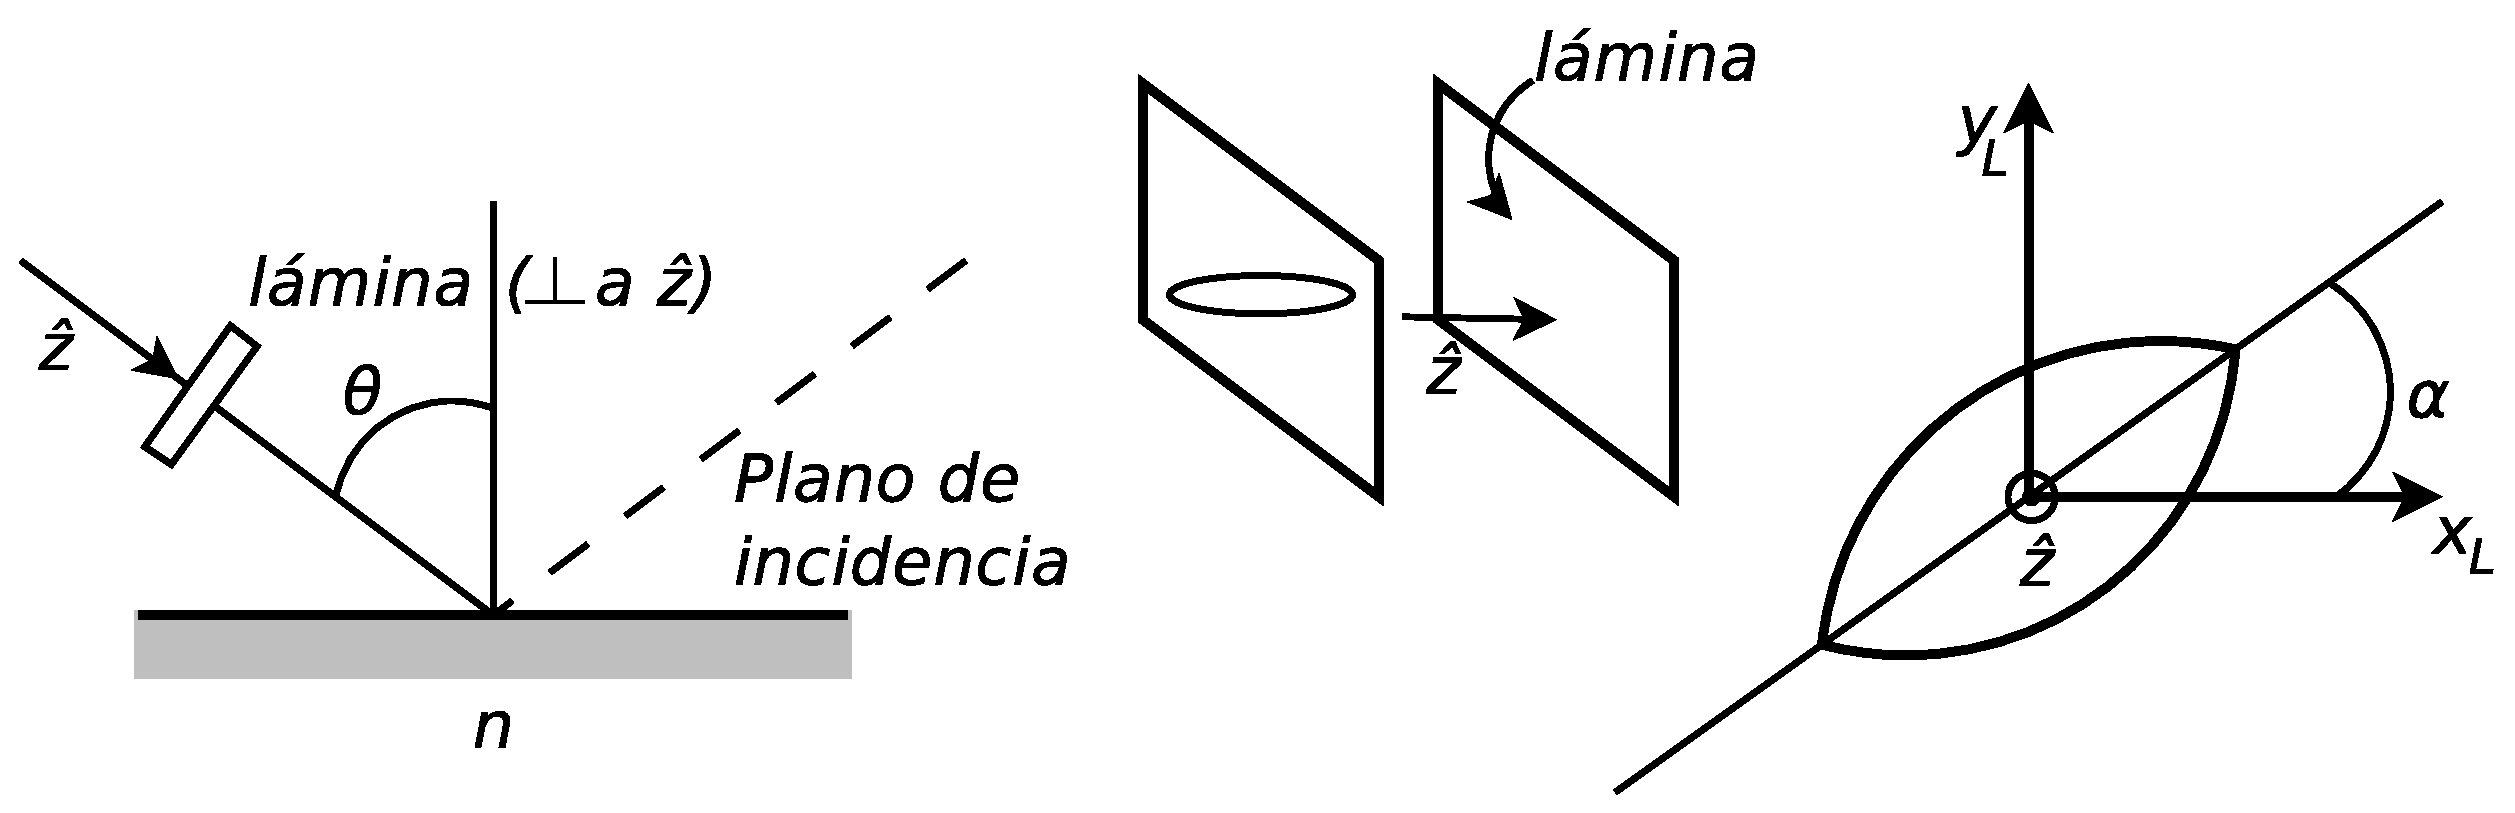
\includegraphics[clip,scale=0.25]{ej4-28}
\end{figure}


\begin{enumerate}
\item ¿Cuál debería ser la polarización del campo a la salida de la lámina
para que esto sea factible? Teniendo esto en cuenta:
\item Diga cómo debe orientarse la fuente con respecto a los ejes de la
lámina. Es decir, halle cuál debe ser el ángulo $\alpha$ formado
entre el eje mayor de la elipse y el eje rápido de la lámina ($x_{L}$).
Halle el campo a la salida de la lámina.

\begin{itemize}
\item halle el ángulo de incidencia ($\theta$)
\item halle el ángulo que debe formar el eje $y_{L}$ de la lámina con la
dirección perpendicular al plano de incidencia. 
\end{itemize}
\end{enumerate}
\begin{description}
\item [{Obs.:}] escriba \uline{claramente} la expresión del campo eléctrico
a la entrada y a la salida de la lámina, indicando el o los sistemas
de coordenadas que usa. \end{description}
\end{enumerate}

\end{document}
